% ==========================================================================
\section{Computer Operation}
% ==========================================================================
    
    % ==========================================================================
    \subsection{dastaZ80DB Front Panel}
    % ==========================================================================
    \label{subsec:frontpanel}

    The dastaZ80DB has a front panel (located for easy access) with buttons,
    switches, indicator lights and a MicroSD slot. Also, in difference to the
    dastaZ80 Original, this computer has a LCD Display and some push buttons
    which form the \textit{Control Panel}.

    The front panel contains:

    \begin{itemize}
        \item ON/OFF Switch: use it to turn on and off the computer.
        \item Micro SD Card slot: for massive storage of data.
        \item Control Panel:
            \begin{itemize}
                \item LCD display: for showing information.
                \item Three push buttons (Up, Down, Select): for operating the
                    Control Panel.
            \end{itemize}
        \item Light (LED) indicators (from left to right):
            \begin{itemize}
                \item Halted (purple): lighted when the system is in \textit{Halt}
                    status.
                \item Bi-colour LED:
                    \begin{itemize}
                        \item Reset (red): lighted when the system is performing
                            a hardware reset.
                        \item ROM Paged (blue): lighted when the \textbf{ROM}
                            chip has been disconnected. Hence, full \textbf{RAM}
                            is available.
                    \end{itemize}
                \item SD card (yellow): blinks when the SD Card is being
                    accessed (reading or writing).
                \item Power (green): lighted when the system is switched ON.
            \end{itemize}
    \end{itemize}

        % ==========================================================================
        \subsubsection{Control Panel}
        % ==========================================================================
        \label{subsubsec:controlpanel}

        This Panel is used to configure some pre-booting configurations (if you
        are familiar with IBM AS/400\footnote{The IBM AS/400 (Application
        System/400) is a family of midrange computers from IBM produced since
        1988.} computers you will see where this idea comes from). It also
        monitors the internal temperature of the box and switches ON and OFF a
        small fan used for cooling.

        The Panel consists of one LCD display and three push buttons. The
        buttons are labelled \textit{+}, \textit{-} and \textit{Select}.

        The LCD displays what is referred in this manual as \textit{pages} of
        information. The buttons \textit{+} and \textit{-} are used to navigate
        the pages, and the button \textit{Select} is used to select a specific
        configuration shown on a page.

        The LCD display is always ON as soon as the computer has been plugged
        to the 5V/4A power supply. That's right, even when the computer is OFF,
        this panel is ON.

        Once the computer is switched ON (via the Power Switch), the
        configuration cannot be changed. Hence, any selection via the
        \textit{Select} button will be ignored.

        Changes in configuration are not stored. Once the computer is unplugged
        from the power supply, it will start again with the default settings.

        \pagebreak

        \textbf{Current Configuration - Page 0}

        When plugged in, the display will show the Page 0. This is indicated by
        the number zero shown in the first character of each of the two lines of
        the display.

        Page 0 shows the Current Configuration. If the computer was to be
        switched ON at this moment, it will use the configuration displayed in
        the LCD to its boot.

        Page 0 information is:
        
        \begin{center}
            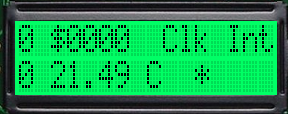
\includegraphics[scale=0.7]{images/dastaZ80_ControlPanel_Page0.png}
        \end{center}

        \begin{itemize}
            \item Line 1:
            \begin{itemize}
                \item \textit{0}: indicates that this is Page 0.
                \item \textit{\$0000}: refers to the address in ROM that will be
                    used to start reading the OS.
                \item \textit{Clk Int}: indicates the the Internal clock is
                    being used as system clock.
            \end{itemize}
            \item Line 2:
            \begin{itemize}
                \item \textit{0}: indicates that this is Page 0.
                \item \textit{21.49 C}: is the current measured internal
                    temperature of the box.
                \item \textit{*}: this only appears if a certain threshold of
                    maximum temperatire has been reached. If the computer is
                    switched ON, here it will appear a spinning animation
                    indicating that the fan is ON. If the computer is OFF, a
                    blinking exclamation mark will appear, indicating that it
                    may not be safe to switch on the computer.
            \end{itemize}
        \end{itemize}

        \textbf{ROM Start Address - Pages 1 and 2}

        Pages 1 and 2 are selectable pages, and show the two different start ROM
        addresses that can be selected.

        The EEPROM that contains the OS can have two different versions. One
        version is burned into the EEPROM at address \texttt{0x0000} and the
        other at \texttt{0x4000}. This is useful for testing new versions or
        even having completely different operating systems.

        \begin{center}
            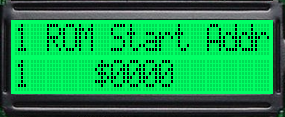
\includegraphics[scale=0.7]{images/dastaZ80_ControlPanel_Page1.png}
            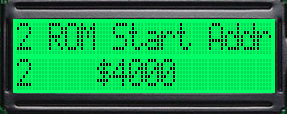
\includegraphics[scale=0.7]{images/dastaZ80_ControlPanel_Page2.png}
        \end{center}

        To select one or the other, press the button \textit{Select} while in
        the desired page. After a couple of seconds, the Panel will display Page
        0 automatically, and you should see the selected value in its
        corresponding position.

        \textbf{HardDisk Drive - Pages 3 and 4}

        Pages 3 and 4 are selectable pages, and show the two different HDD that
        can be selected.

        The two options are:

        \begin{itemize}
            \item \textbf{Internal HHD}: This is the Sd Card controlled by the
                \textbf{ASMDC}, and consist of a MiniSD card slot that allows
                the insertion/extraction of MiniSD cards containing Disk Image
                Files.
            \item \textbf{External HDD}: At the back of the computer, there is a
                6-pin header to which an FTDI-to-USB cable can be connected. On
                a PC, connected to the USB end of the cable, a program (called
                \textit{SerialHDDsimul}) can be run and simulate the behaviour
                of the \textbf{ASMDC}, but with 3.8 times faster access.
        \end{itemize}

        % \begin{center}
        %     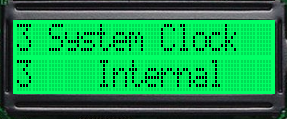
\includegraphics[scale=0.7]{images/dastaZ80_ControlPanel_Page3.png}
        %     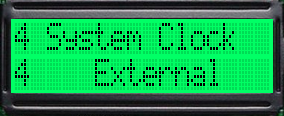
\includegraphics[scale=0.7]{images/dastaZ80_ControlPanel_Page4.png}
        % \end{center}

        \textbf{Video Output - Pages 5 and 6}

        Pages 5 and 6 are selectable pages, and show the two different video
        output that can be selected.

        You MUST change this configuration accordingly to how you did set up the
        computer (as explained in the section \hyperref[sec:setting_system]
        {Setting up the system}). Select \textit{TTL Serial} if you are using
        a TTL-to-USB (or TTL-to-RS-232) cable for input and output, or Select 
        \textit{VGA} if you are using TTL-to-USB (or TTL-to-RS-232) cable for
        input but VGA for output.

        \begin{center}
            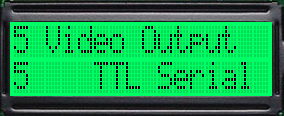
\includegraphics[scale=0.7]{images/dastaZ80_ControlPanel_Page5.png}
            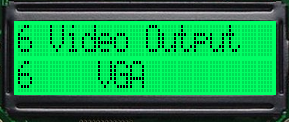
\includegraphics[scale=0.7]{images/dastaZ80_ControlPanel_Page6.png}
        \end{center}

    \pagebreak
    
    % ==========================================================================
    \subsection{ON/OFF button}
    % ==========================================================================
    \label{subsec:onoffbutt}

    The ON/OFF button is located on the lefthand side of the back of the
    dastaZ80 computer and on the front of the dastaZ80DB.

    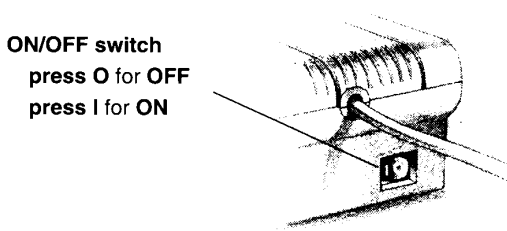
\includegraphics[scale=0.5]{images/onoffbutton.png}

    This button is used to turn ON and OFF the computer.

    Before turning it ON, read the instriuctions on the section
    \hyperref[sec:setting_system]{Setting up the system} of this manual.

    Before turning it OFF, it is highly recommended to use the command 
    \hyperref[cmd:halt]{halt} to ensure that all \textbf{DISK} data has been
    correctly saved. Otherwise, corruption of data may occur.

    % ==========================================================================
    \subsection{Reset button}
    % ==========================================================================
    \label{subsec:resetbutton}

    The reset button is located on the lefthand side on both the dastaZ80 and
    the dastaZ80DB.

    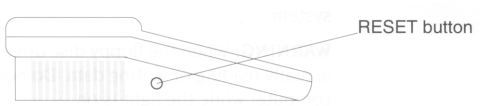
\includegraphics[scale=0.7]{images/resetbutton.png}

    To reset the computer simply press and release the button.

    When pressed, the internal Reset Circuit sends a reset signal to all chips
    in the computer, and thus setting them to an initial and unconfigured state.
    One of those chips is the CPU itself, which when reset or powered ON starts
    executing code found at the very beginning of the \textbf{ROM}, and hence
    re-configuring all chips. In the section appendix \textit{OS Boot Sequence}
    of the \textit{dastaZ80 Programmer's Reference Guide}\cite{dastaz80progref}
    there is detailed information of what happens after a reset or power up.

    The reset process will take 6.5 seconds in total, as explained in the
    section \textit{Reset circuit} of the \textit{dastaZ80 Technical Reference
    Manual}\cite{dastaz80techman}.

    % ==========================================================================
    \subsection{Indicator LEDs}
    % ==========================================================================

    Indicator LEDs for the dastaZ80DB has been discussed in previous section
    \hyperref[subsec:frontpanel]{dastaZ80DB Front Panel}.

    For the dastaZ80, at the top of the computer case there a few labelled
    LEDs that give information of the  status of several internal parts of the
    computer.

    \begin{itemize}
        \item Above the numeric pad, on the righthand side of the keyboard,
        there are two LEDs:
        \begin{itemize}
            \item \textbf{POWER}. This LED is always on when the computer is
            switched on via the \hyperref[subsec:onoffbutt]{ON/OFF button}. It glows
            in \underline{orange} colour.
            \item \textbf{DISC}. This LED blinks whenever a \textbf{DISK} operation
            (read/write) is happening. It glows in \underline{green} colour.
        \end{itemize}
    \end{itemize}
    
    \centerline{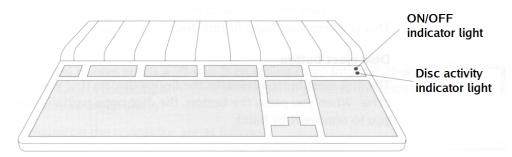
\includegraphics[scale=0.5]{images/keyboardLEDs.png}}

    \begin{itemize}
        \item Above the \textit{Esc} and function keys (\textit{F1}-\textit{F12}),
        on the lefthand side of the keyboard, there are two LEDs. These LEDs are
        multi-colour, hence glowing at different colour each:
        \begin{itemize}
            \item Computer status
            \begin{itemize}
                \item \textbf{RESET}. Lighted in \underline{red} colour when
                the computer is in reset status. This happens for 6.5 seconds
                when the computer is switched ON (via the
                \hyperref[subsec:onoffbutt]{ON/OFF button}) and when the
                computer is reset via the \hyperref[subsec:resetbutton]
                {Reset button}.
                \item \textbf{HALTED}. Lighted in \underline{purple} when the
                computer is in halt status. Usually after issuing the command
                \hyperref[cmd:halt]{halt}.
                \item \textbf{ROM PAGED}. Lighted in \underline{blue} when the
                \textbf{ROM} has been electrically disconnected and therefore
                the computer will only perform operations (read/write) from/to
                the \textbf{RAM}. This happens only during the Boot Sequence.
                See the section \textit{OS Boot Sequence} of the dastaZ80
                Programmer's Reference Guide\cite{dastaz80progref} for more
                detailed information about the Boot Sequence.
            \end{itemize}
            \item Clock Selection
            \begin{itemize}
                \item \textbf{CLOCKSEL}. It glows in \underline{yellow} colour
                when the Internal clock is used. And in \underline{purple}
                colour when an External clock is being used by the computer.
            \end{itemize}
        \end{itemize}
    \end{itemize}

    % ==========================================================================
    \subsection{MicroSD}
    % ==========================================================================

    At the back of the dastaZ80 computer and on the front of the dastaZ80DB
    there is a MicroSD slot.

    Insert here a MicroSD formatted with FAT32 and containing Disk Image
    Files formatted with DZFS\footnote{DZFS (dastaZ80 File System) is a file
    system of my own design, for mass storage devices, aimed at simplicity}.

    \centerline{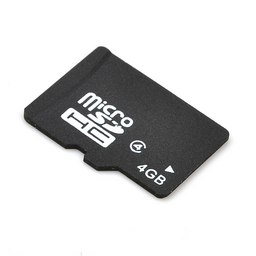
\includegraphics[scale=0.5]{images/microsdcard.png}}

    % ==========================================================================
    \subsection{3.5 inch Floppy Disc Drive}
    % ==========================================================================

    The Floppy Disc Drive is located on the righthand side of the dastaZ80
    computer and on the front of the dastaZ80DB.

    3.5 inch floppy discs can be inserted in this drive. 

    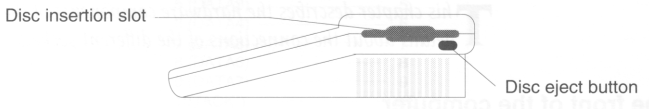
\includegraphics[scale=0.7]{images/discslot.png}

    To remove an inserted floppy disc from the drive, press the
    \textit{Disc eject button}. The disc will partially pop out, allowing you to
    completelly remove it by hand.

    % ==========================================================================
    \subsection{Attaching peripheral devices}
    % ==========================================================================

        % ==========================================================================
        \subsubsection{TTL I/O}
        % ==========================================================================
        \label{subsubsection:ttlio}

        The dastaZ80DB has a 6-pin header labelled \textit{TTL I/O} that is
        used for connecting either a TTL-to-USB cable or a TTL-to-RS232
        converter.

        This connector carries the signals for the input (keyboard) and output
        (screen).

        By connecting the dastaZ80DB to another computer, the latter can
        \textit{control} the former. As a matter of fact, there is no other way
        to input commands to the dastaZ80DB than using another device (a
        computer in most cases, but also a serial terminal can be used).

        For the output, two options are available:

        \begin{itemize}
            \item \textit{TTL}: output to a serial device (usually another
                computer running a terminal program).
            \item \textit{VGA}: output to a VGA monitor.
        \end{itemize}

        The option \textit{VGA} MUST be selected in the page 6 (Video Output) of
        the \hyperref[subsubsec:controlpanel]{Control Panel}).

        The TTL connector pins are configured as follows (seeing it from the
        front):

        \textbf{Ground} | NC | NC | \textbf{TX} | \textbf{RX} | NC

        NC, stands for Not Connected. These are the \textit{+5V}, \textit{/CTS}
        and \textit{/RTS} signals, which are not used.

        % ==========================================================================
        \subsubsection{Dual Video Output}
        % ==========================================================================

        At the back of the computer you will find two connectors, beside each
        other, for the connection of video output.

        The first one, and necessary to use the computer, is a VGA connector for
        the \textbf{VGA video output}.
        
        Plug here a standard VGA cable connected to a VGA monitor.

        \centerline{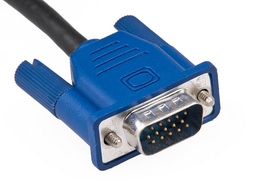
\includegraphics[scale=0.5]{images/vgaconn.png}}

        The second connector, which is optional (i.e. the computer will function
        perfectly normal without this connected), is a 3.5mm female jack for the
        NTSC \textbf{Composite video output}.

        Plug here the jack side of a 3.5mm jack-to-3-RCA Audio/Video cable
        \footnote{This is the same cable used on the Raspberry Pi for Composite
        output.}.

        \centerline{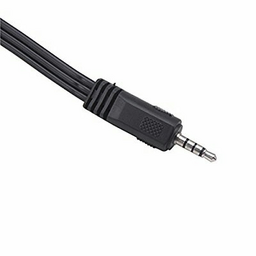
\includegraphics[scale=0.5]{images/raspicable_jack.png}}

        Connect the yellow RCA cable of the jack-to-3-RCA cable to the Composite
        input of a monitor or TV.

        \centerline{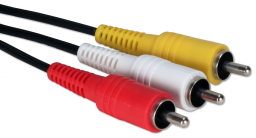
\includegraphics[scale=0.5]{images/raspicable_rca.png}}

        % ==========================================================================
        \subsubsection{Stereo Sound Output}
        % ==========================================================================

        The stereo sound signal comes out of the same connector used for the
        Composite video output.

        Connect the jack-to-3-RCA white and red cables to a pair of speakers or
        to the input of a sound system amplifier.

        % ==========================================================================
        \subsubsection{USB Keyboard for External computer}
        % ==========================================================================

        The keyboard of the dastaZ80 can be used as an USB keyboard on other
        computers.
        
        Connect the a USB cable between this connector and your other
        computer, switch on dastaZ80 and press the key \textit{ScrollLock}. From
        now on (as indicated by the ScrollLock LED being lighted) dastaZ80 will
        not read any keystrokes, but instead will send them to the computer
        connected via USB.

        If you want to use dastaZ80 at any time, just press \textit{ScrollLock}
        again. There is no need to unplug the USB cable. The \textit{ScrollLock}
        key is doing the switching.

        This feature can be handy when you are using dastaZ80 and another PC at
        the same time and don't want to be switching hands between two keyboards
        all the time. It saves space too!

        % ==========================================================================
        \subsubsection{ROM Cartridge}
        % ==========================================================================

        Refer to the section \textit{Cartridge Port} of the dastaZ80 Technical
        Reference Manual\cite{dastaz80techman} for more detailed information.

        % % ==========================================================================
        % \subsubsection{General-Purpose Input/Output (GPIO)}
        % % ==========================================================================

        % This connector exposes all CPU signals and can be used to connect external
        % devices directly to the components (e.g. \textbf{CPU}, \textbf{RAM)} of
        % the computer.

        % ==========================================================================
        \subsubsection{External HDD}
        % ==========================================================================

        The dastaZ80DB has a 6-pin header labelled \textit{External HDD} that is
        used for connecting either a TTL-to-USB cable or a TTL-to-RS232
        converter.

        This connector carries the signals for the Transmit (\textit{TX}) and
        receive (\textit{RX}) of an external \textbf{DISK} device.

        By connecting the dastaZ80DB to another computer, the latter can provide
        a fast hard disk drive simulation (3.8 times faster than the SD Card on
        the \textbf{ASMDC}).

        The option \textit{External} MUST be selected in the page 4 (HardDisk
        Drive) of the \hyperref[subsubsec:controlpanel]{Control Panel}).

        The TTL connector pins are configured as follows (seeing it from the
        front):

        \textbf{Ground} | NC | NC | \textbf{TX} | \textbf{RX} | NC

        NC, stands for Not Connected. These are the \textit{+5V}, \textit{/CTS}
        and \textit{/RTS} signals, which are not used.

    % ==========================================================================
    \subsection{Developer Mode}
    % ==========================================================================
    \label{subsec:devmode}

    At the back of the dastaZ80 is located a pin header that configures the
    routing of the signals between the the serial device and the internal I/O
    devices.

    By default, the signals are routed as follows:

    \begin{itemize}
        \item Serial TX $\rightarrow$ VGA controller RX
        \item Serial RX $\leftarrow$ Keyboard controller TX
    \end{itemize}

    It's possible to redirect these signals to an external device (e.g. a
    computer running a terminal emulator software like Minicom or PuTTY). This
    configuration allows to use the computer via an external keyboard and/or
    outputting the video signal to that device.

    In the dastaZ80DB, this pin header is the \hyperref[subsubsection:ttlio]
    {TTL I/O}, and signals are not routed because is used for connecting either
    a TTL-to-USB cable or a TTL-to-RS-232 converter.

    It's called \textit{Developer Mode}, because with this configuration is very
    easy (and quick), to send programs via the \hyperref[software:pastefile]
    {pastefile} tool and test them. Basically, we can write programs directly to
    the \textbf{RAM}, without the need of transfer them to the MicroSD card.